\scanpage{105}
\mspage{104}%
par un $H'$-torseur à \rlap{droite}gauche $Q$.

Moyennant la vérification laissée en suspens à l'instant, on trouve alors que la donnée d'un``foncteur fibre \uline{filtré}''$F$ de $\underline{C}$ sur $k$ revient à la donnée

(i) d'un foncteur fibre $F'$ \deleted{gradué de type} (d'où un groupe\deleted{d} de Galois $G'=\underline{\operatorname{Aut}}(F')$ );\rlap{\tikz[baseline=0pt,x=1em,y=1em]{\draw (0,-.5)--(.03,-.65);}}

(ii) D'une grad\rlap{d}uation de type $\underline{Z}$ de $F'$, i.e. un homomorphisme
\[
i_1:\underline{G}_m\handwritten{\longrightarrow}G',
\]
\margin{\tikz[baseline=0pt,x=1em,y=1em]{\draw (0,0)--(.12,.2)--(.08,.3);}}ce qui permet de définir comme ci-dessus un sous-groupe $H'_{i_1}$ de $G'$ ;

(iii) D'un torseur à \rlap{droite}gauche $Q'$ sous $H'_{i_1}$.

A ces données, on associe simplement le foncteur fibre tordu
\[
F=F'\mathop{\handwritten{\wedge}}\limits^{H'_{i_1}}Q',
\]
$F$ étant filtré par la filtration déduite de celle de $F'$ \deleted{(\unsure{via} la \unsure{graduatio|graduation}} (associée à la graduation de $F'$) en tordant par $Q'$.

\deleted{NB Dans le cas où $F$ est le foncteur de De Rham sur la catégorie des motifs sur $k$, on prouve (moyennant le yoga général des motifs - il est possible qu'on utilise pour ceci les conjectures de Hodge ...) que le groupe $H'$ est une limite projective de groupes algébriques \deleted{\inserted{lisses}} \deleted{à composantes connexes \uline{résolubles}\unsure{.} Donc}\inserted{unipotents} \unsure{$\mathbb{S}$|S}i on se borne à une catégorie de motifs \deleted{de} à engendrement fini, et si $G$ est connexe, on trouve aussi que $H'$ est connexe, donc étant résoluble, on trouve}

On constate aisément que le groupe $H'$ est nécessairement une limite projective de groupes algébriques \uline{unipotents}. On en conclut aussitôt que si $\underline{C}$ est à engendrement fini (ou, plus généralement, \inserted{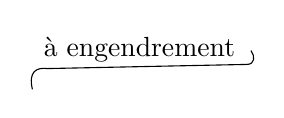
\begin{tikzpicture}[baseline=-.2ex,x=1em,y=1em]
\node[anchor=base west] at (0,.5) {\handwritten{à \unsure{engendrement}}};
\draw (-.05,-.7) .. controls (-.2,-.05) and (.1,.1) .. (.5,.05) -- (7.7,.2) .. controls (8,.2) and (8,.5) .. (7.85,.7);
\end{tikzpicture}} dénombrable, de façon que $G'$ \deleted{soit} donc aussi $H'$ soit limite projective d'une \uline{suite} de groupes algébriques)\margin{\tikz[baseline=0pt,x=1em,y=1em]{\draw (0,0)--(.16,.2);}} alors tout torseur sous $H'$ est trivial; cela signifie ici que tout foncteur fibre filtré est en fait associé à un foncteur fibre gradué (en prenant la filtration correspondant à la graduation)

